\chapter{Azure IoT Hub}

The Azure suite is Microsoft's solution for cloud computing. It contains a host of options for data acquisition, storage, processing and analytics, and visualization and display. Each option is called a resource.

\todo[inline]{Had a different diagram in mind, replace if you find it}

\begin{figure}[H]
\centering
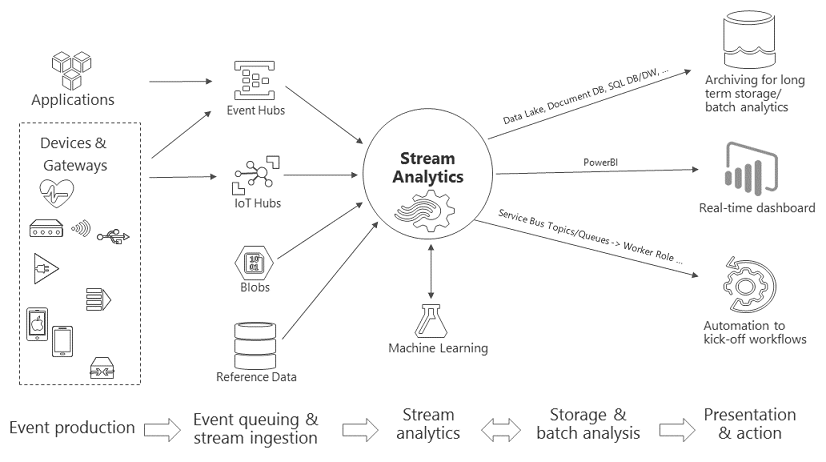
\includegraphics[scale=0.65]{Images/stream_analytics_intro_pipeline.png}
\caption{Example Azure network of resources \\ Source/courtesy of: https://docs.microsoft.com/en-us/azure/stream-analytics/stream-analytics-introduction}
\label{fig:exampleNetwork}
\end{figure}

The different services of Azure can be broken down into several overall layers, based on their specific function. Each component can be mixed and matched to create a unique data processing network.

\section{Connection to IoT Hub}
The ReVolt Model makes use of the iothub-client python library to connect to the IoT Hub. Messages are created as strings and sent using the built-in functions at a desired rate set by the publisher in ROS. The data to send is sampled at a rate of 20 Hz. However, since there is a limit and price based on number of messages sent and not based on the size of the messages, the data samples are packaged into 1 message and the messages are sent at a slower rate, currently 1 Hz. This is not an issue for twin mode visualization, as that data is sent directly to the Unity Application without the use of Azure. The messages arrive at the IoThub in json format.

\section{Stream Analytics and Storage}
\todo[inline]{reorganize this whole section}
\todo[inline]{add figure with just Azure resources that I'm using}
Incoming data is processed in two different ways, on a hot and cold data path. A hot path refers to a data stream that processes data with no relation to the previous data. In this case, the data are the realtime information coming from the ReVolt model. Since data is instead being sent directly to the ReVolt model through a TCP web socket, no hot path is used currently. However, future work could include analytics of the incoming data for anomolys.

The cold path refers to data which will be analyzed as a whole, and in retrospect, using big data techniques. Analysis does not occur on-the-fly, so the most important step is storing the data. The data is stored in an SQL Database in the Azure service. In order to accomplish this, a stream analyitics resource is used. Azure's Strsm Analytics resources are simple ways to connect incoming data streams with data sinks, all while processing the data in between. In this case, the input stream is the IoT device (the ReVolt model) and the output sink is the Azure SQL Database. The stream analytics resource takes care of unpacking each sample of data, as the data samples have been packaged and sent at a lower frequency to reduce the number of messages sent. Each sample of data is placed in a unique row in the SQL table. This path is highlighted in \Cref{ADD REFERENCE!!!}. 

In the Unity Application's Playback mode, the data from the database is retrieved to visualize certain specific events. This is accomplished using a webform which runs a php script hosted on an Azure web app. This filters and returns all of the relavant data from the SQL Database as a formated string, which is parsed by unity for playback.

The data sent is currently as follows:
\todo[inline]{add table of data}
Future work will include refinement of what data is needed from ReVolt in order to perform analytics.





